\documentclass[utf8]{beamer}

\usetheme{default}
\usecolortheme{seagull}
\usefonttheme{serif}

\usepackage{graphicx}
\usepackage{amsmath}
\usepackage{bm} % bold math symbols
\usepackage{tgpagella} % Gyre pagella -- based on palatino
\usepackage[english]{babel}
\usepackage[binary-units]{siunitx}

../text/math-defs.tex

\title{Exploiting GPS in Monte Carlo Localization}
\author{Jakub Marek}


\newcommand{\imageframe}[1]{
{
\hspace{-1.36cm}
\setbeamercolor{background canvas}{bg=black}
\begin{frame}[plain]
    \begin{centering}
        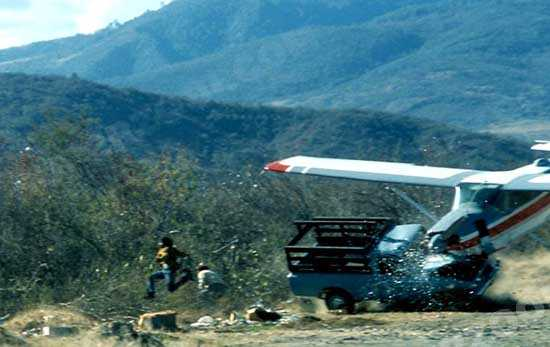
\includegraphics[width=\paperwidth,height=\paperheight,keepaspectratio]{img/01.jpg}
    \end{centering}
\end{frame}
}
}


\begin{document}


\begin{frame}[plain]
    \titlepage
\end{frame}


\section{Motivation}
\begin{frame}{Motivation}
    \begin{itemize}
        \item Outdoor robots need position information
        \item GPS looks promissing
        \begin{itemize}
            \item Worldwide absolute position
            \item No preparation required
         \end{itemize}
        \item \ldots but it has its drawbacks
        \begin{itemize}
            \item Low precision from consumer GPS receivers
            \item Low measurement frequency
         \end{itemize}
        \item Attempt to improve precision from GPS
        \begin{itemize}
            \item Combination with other sensors
         \end{itemize}
    \end{itemize}
\end{frame}

\imageframe{img/01.jpg}

\section{GPS}
\begin{frame}{GPS}
    \begin{itemize}
        \item Global satellite navigation system
        \item Measuring time of flight of radio signals
        \begin{itemize}
            \item Ideally: position = intersection of spherical surfaces
            \item In fact: 4D conical surfaces (3D positions + clock offsets)
        \end{itemize}
        \item Pseudorange
        \begin{itemize}
            \item \(\rho = \speedoflight (\recrxtime - \svtxtime)\)
            \item Distance corresponding to time of flight
            \begin{itemize}
                \item Transmission time according to satellite clock
                \item Receipt time according to receiver clock
            \end{itemize}
        \end{itemize}
        \item Doppler measurements
        \begin{itemize}
            \item Relative velocities of satellite and receiver
        \end{itemize}
    \end{itemize}
\end{frame}

\section{Monte Carlo Localization}
\begin{frame}{Monte Carlo Localization}
    \begin{itemize}
        \item Probabilistic localization algorithm
        \item Simple to understand and implement
        \begin{itemize}
            \item Simulating a swarm of possible robots
            \item Comparing the actual and simulated sensor readings
        \end{itemize}
        \item Only requires probability of a measurement
        \item More computationaly intensive than e.g. Kalman Filter
    \end{itemize}
\end{frame}

\section{GPS with MCL}
\subsection{Simple Approach}
\begin{frame}
    \frametitle{GPS with MCL -- simple approach}
    some text
\end{frame}

\begin{frame}
    \frametitle{GPS with MCL -- simple approach}
\end{frame}

\subsection{Low Level Approach}
\begin{frame}
    \frametitle{GPS with MCL -- low-level approach}
\end{frame}

\begin{frame}
    \frametitle{GPS with MCL -- low-level approach}
\end{frame}

\begin{frame}
    \frametitle{GPS with MCL -- low-level approach}
\end{frame}

\begin{frame}
    \frametitle{GPS with MCL -- low-level approach}
\end{frame}

\end{document}
